Työssä tutkittiin sekä vanhan että uuden kaatoratkaisun pohjalta saatuja tuloksia kaatojen määrissä, jotta niitä voitaisiin vertailla. Kaatoja tehtiin 4 cl, 10 cl, 16 cl ja 20 cl kokoisilla tilauksilla ja kaikki kaadot tehtiin vedellä. Samalla jokaisen kaadon välissä punnittiin pullossa jäljellä oleva neste, jotta voidaan huomioida sen vaikutus kaadon määrään. Ideaalisesti pullossa olevan nesteen määrä ei vaikuttaisi kaadon määrään. Tässä kappaleessa on esitetty kuvaajat, joissa on tulokset juomien kaadolle sekä vanhaa että uutta kaatotapaa käyttäen. Kuvissa \ref{fig:kaadot_vanha} ja \ref{fig:kaadot_uusi} esitetyissä kuvaajissa on x-akselilla pullossa olevan nesteen määrä ennen kaatoa ja y-akselilla lasiin saatu juoman määrä.

\begin{figure}[h]
\begin{center}
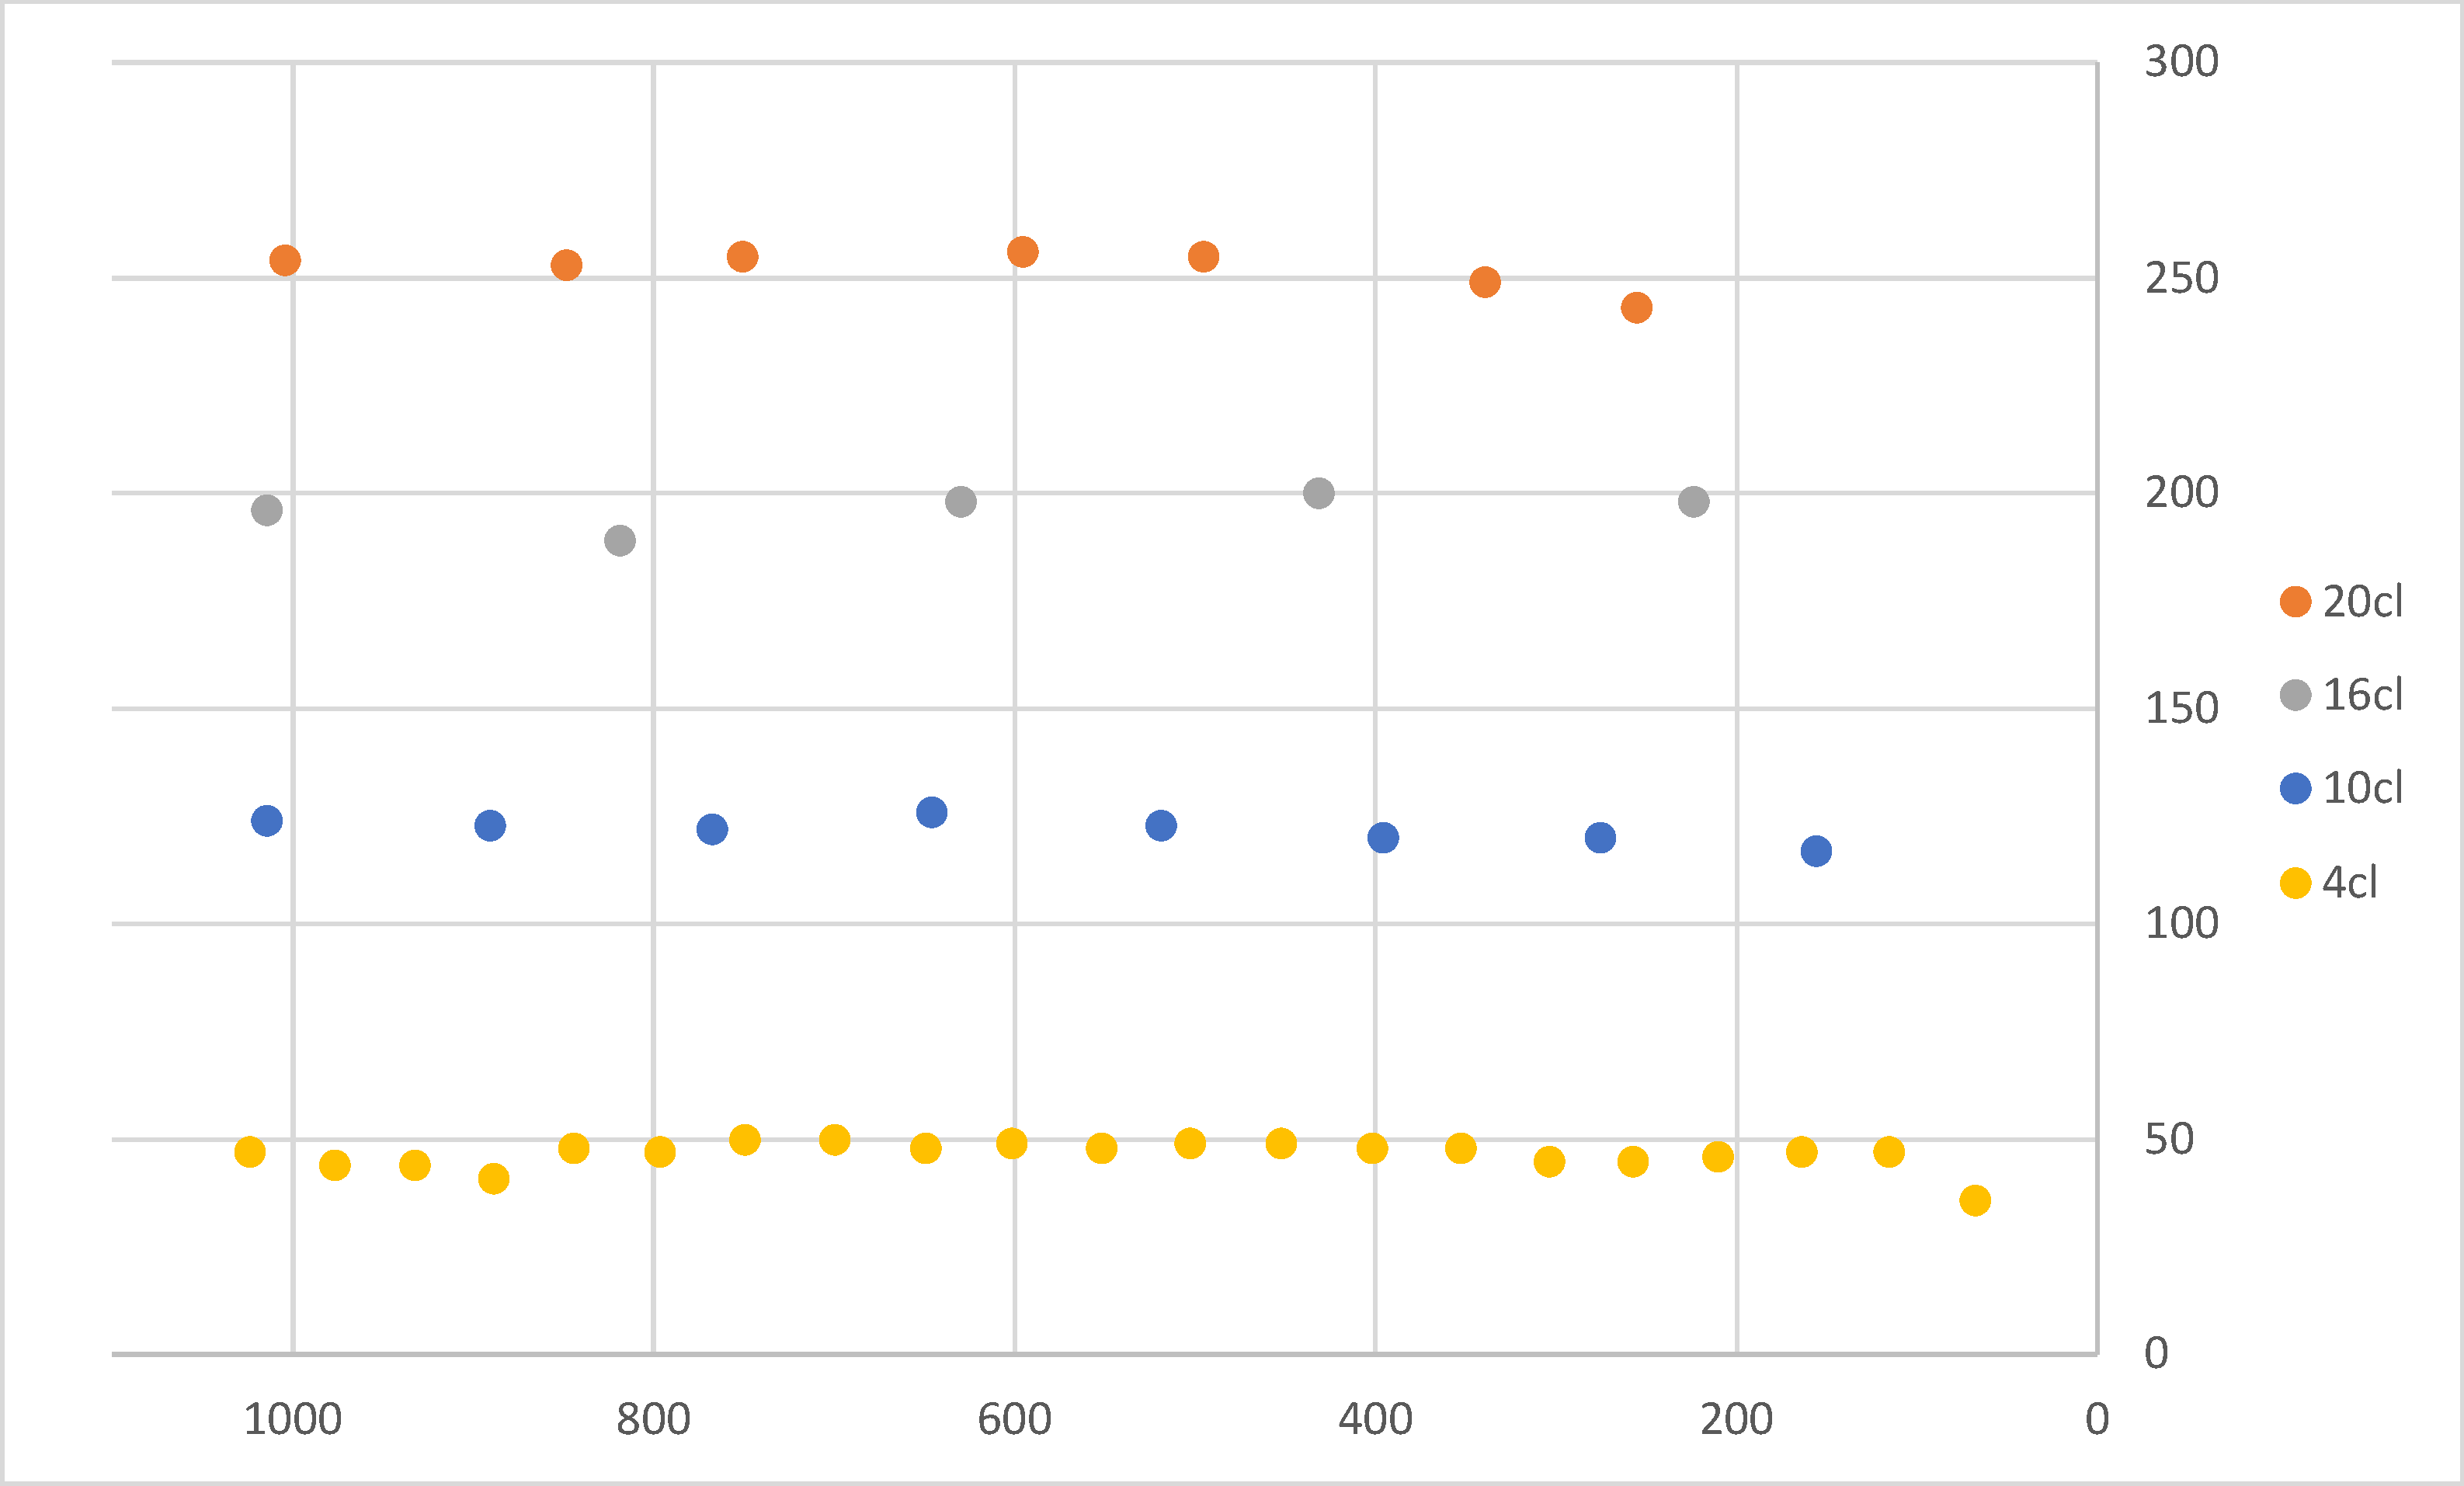
\includegraphics[scale=0.25]{img/kaadot_vanha.pdf}
\end{center}
\caption{Vanhalla kaatoratkaisulla saadut tulokset}
\label{fig:kaadot_vanha}
\end{figure}

Kuten kuvassa \ref{fig:kaadot_vanha} olevasta vanhan kaatoratkaisun tulosten kuvaajasta huomataan, varianssia oli kohtalaisen paljon. Saadut juomamäärät laseissa eivät olleet tasaisia, vaan joka kaadolla ne muuttuivat hieman. Esimerkiksi 4 cl tilauksessa suurin saatu juomamäärä oli noin 50 grammaa ja pienin n. 36 grammaa. 20 cl tilauksessa suurin saatu juomamäärä oli noin 255 grammaa ja pienin n. 214 grammaa. Näiden välinen ero on huomattava, varsinkin kun tarkastellaan eron prosentuaalista osuutta halutusta juomamäärästä.

Kuvaajassa olevista tuloksista saadaan myös vahvistus väitteelle, että pullossa jäljellä oleva juomamäärä vaikuttaa saatuun juoman määrään. Usealla kaatomäärällä mukiin saatu määrä vaihtelee ensin satunnaisesti tietyllä välillä, mutta käyrän loppupää kääntyy alaspäin. Tästä voidaan päätellä, että pullosta, jossa on vain vähän yli tarvittava määrä juomaa, virtaa sitä hitaammin kaadon lopussa.

Sen lisäksi, että saadut juomamäärät vaihtelevat keskenään paljon ja pullossa oleva juomamäärä vaikuttaa saadun juoman määrään, kaatomäärät ovat myös keskimäärin liian suuria. Koska jokaisella kaatomäärällä juomaa on tullut liikaa suhteessa tilattuun määrään, voidaan päätellä että vanhan funktion kulmakerroin on ollut liian suuri.

\begin{figure}[h]
\begin{center}
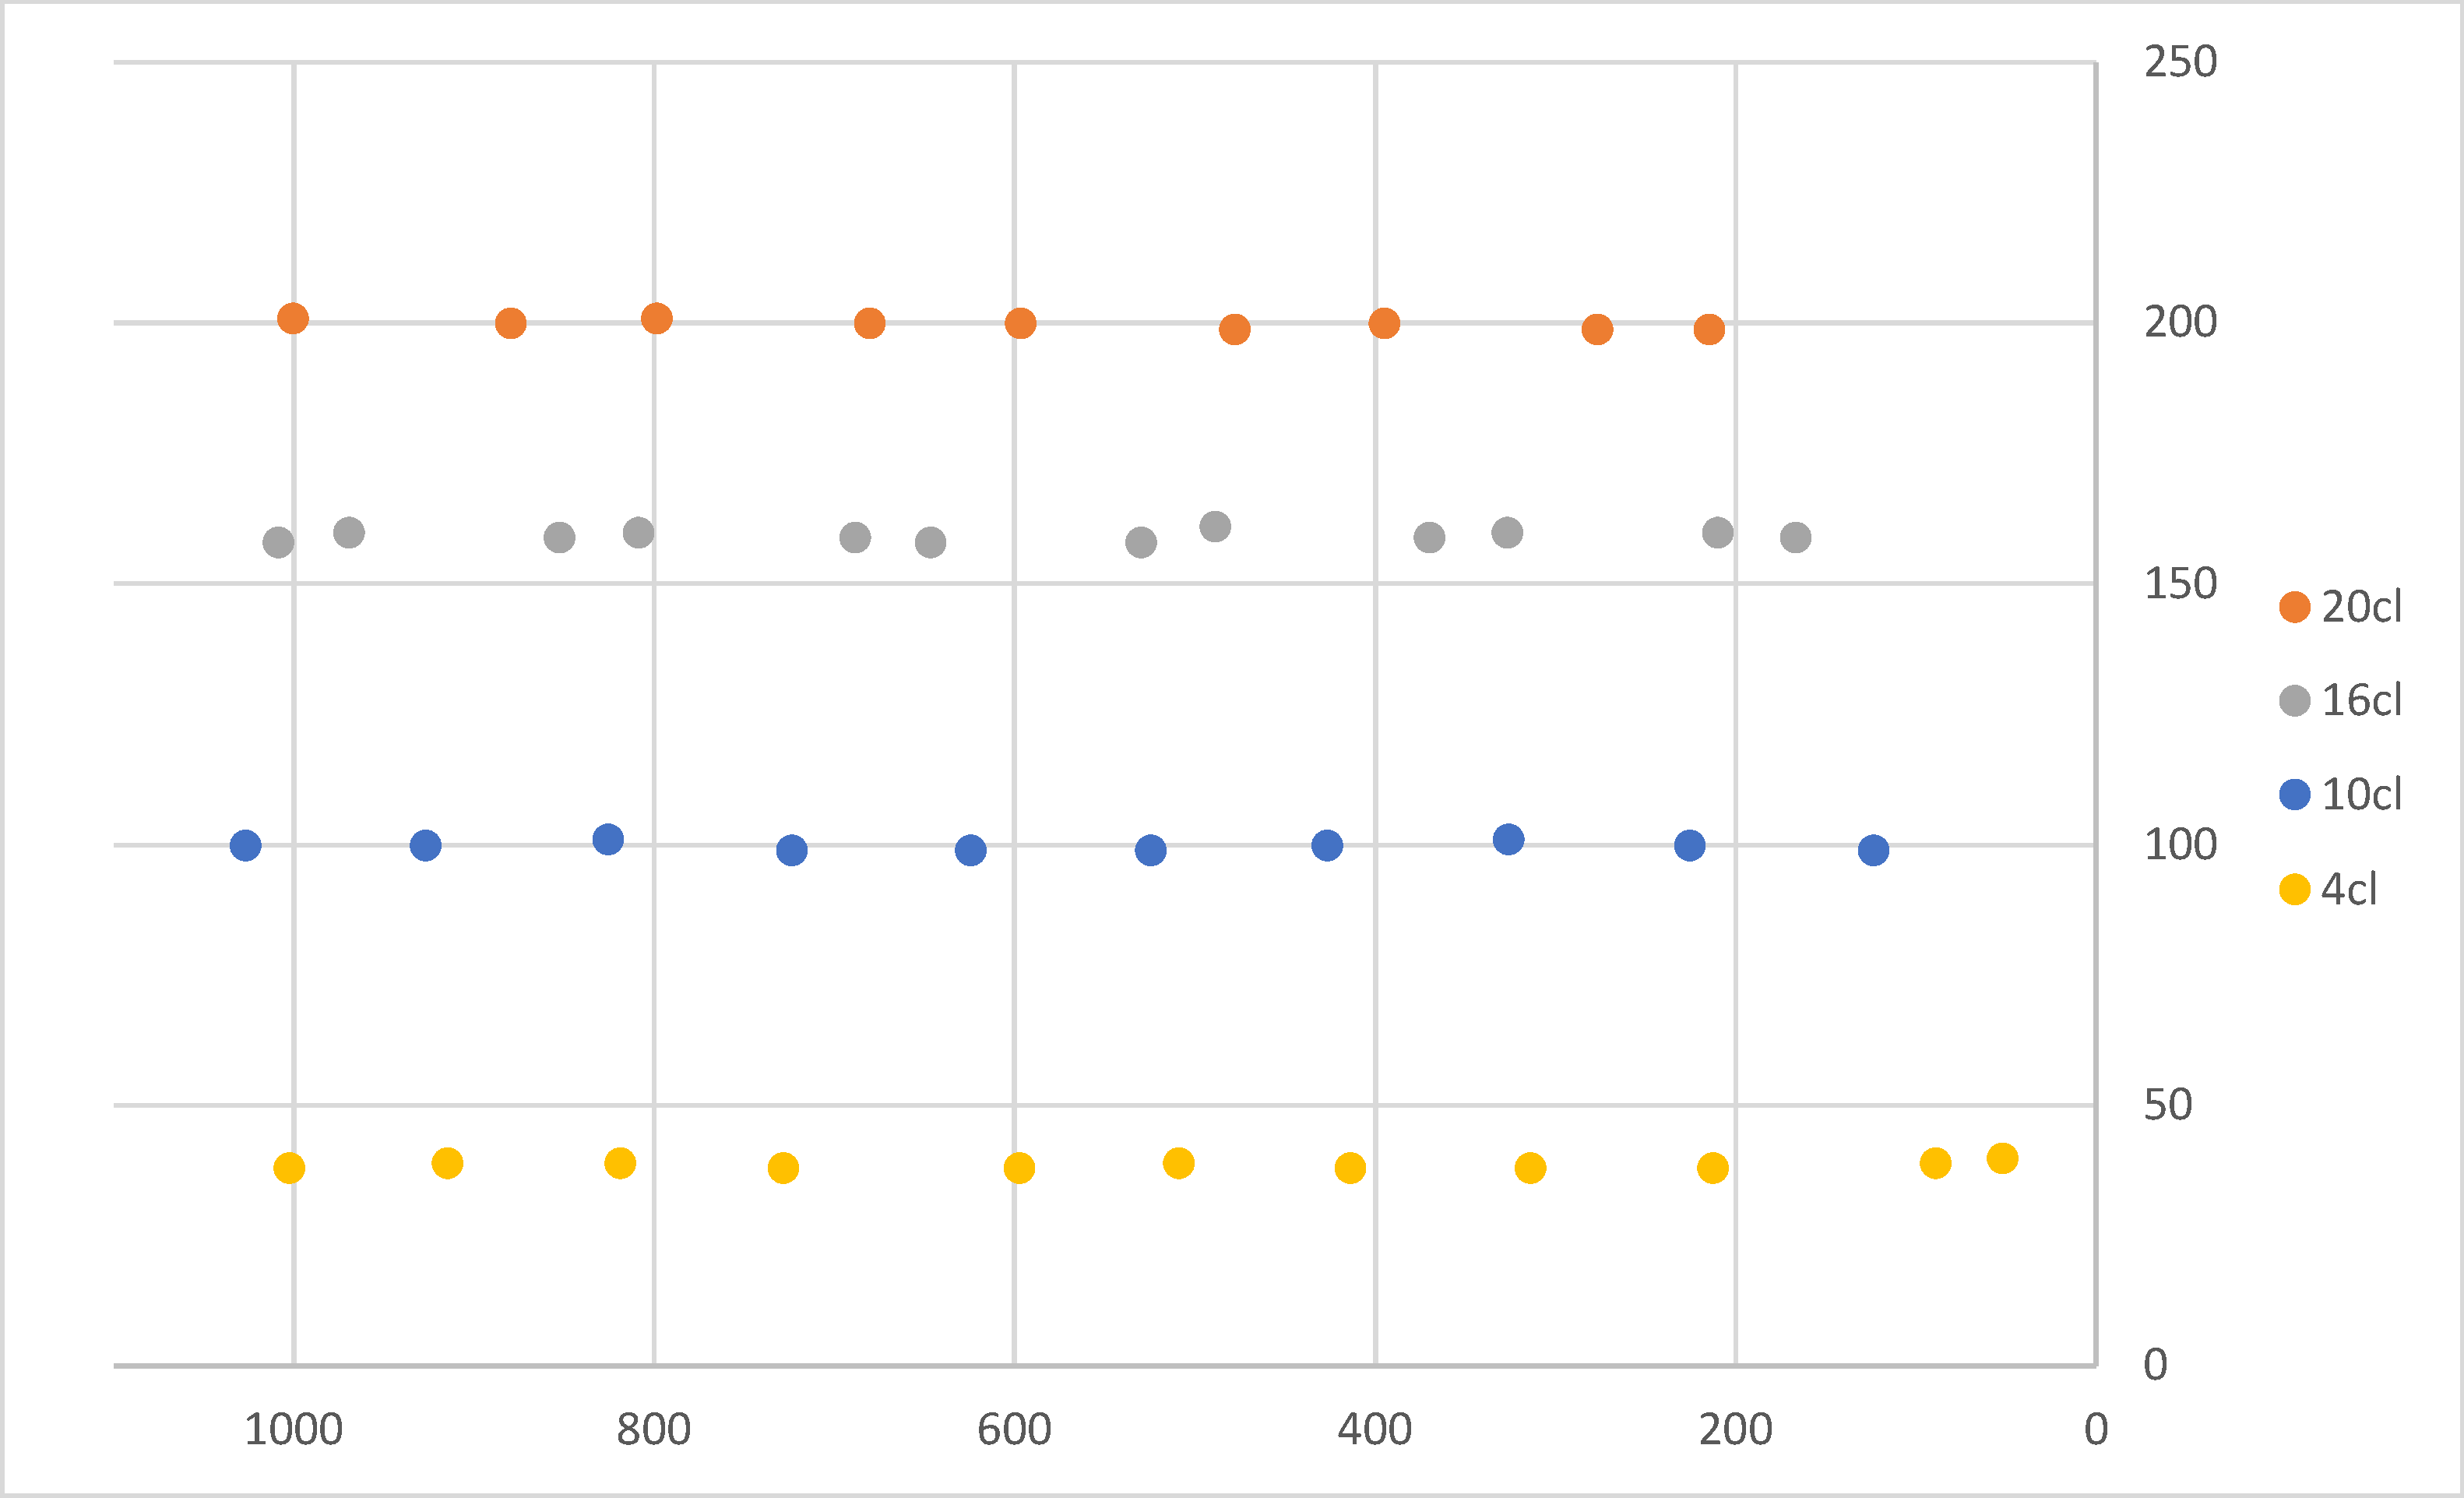
\includegraphics[scale=0.25]{img/kaadot_uusi.pdf}
\end{center}
\caption{Uudella kaatoratkaisulla saadut tulokset}
\label{fig:kaadot_uusi}
\end{figure}

Kuten nähdään uudella kaatoratkaisulla saaduista tuloksista kuvassa \ref{fig:kaadot_uusi}, uusi kaatoratkaisu on huomattavasti tarkempi. Siinä kaatomäärät vaihtelevat korkeintaan yhdellä grammalla eikä niihin vaikuta pullossa ennen kaatoa oleva juoman määrä.
